\documentclass[12pt,a4paper]{article}

\usepackage[margin=1in]{geometry}
\usepackage{graphicx}
\usepackage{xcolor}
\usepackage{setspace}
\usepackage{fancyhdr}
\usepackage{titlesec}
\usepackage{enumitem}
\usepackage{hyperref}
\usepackage{float}
\usepackage{booktabs}
\usepackage{longtable}
\usepackage{array}
\usepackage{amsmath}

\definecolor{answerblue}{RGB}{0,70,170}

\hypersetup{
    colorlinks=true,
    linkcolor=black,
    urlcolor=black,
    citecolor=black
}

\pagestyle{fancy}
\fancyhf{}
\fancyhead[L]{Data Mining (Graduate Level)}
\fancyhead[R]{Spring 2026}
\fancyfoot[C]{\thepage}

\titleformat{\section}
{\large\bfseries\color{black}}
{\thesection.}{0.5em}{}

\titleformat{\subsection}
{\normalsize\bfseries\color{black}}
{\thesubsection.}{0.5em}{}

\titleformat{\subsubsection}
{\normalsize\bfseries\color{black}}
{\thesubsubsection.}{0.5em}{}

\setstretch{1.15}
\setlength{\headheight}{15pt}

\newcommand{\qtext}[1]{\noindent\textbf{#1}\par}
\newcommand{\ansstart}{\begingroup\color{answerblue}}
\newcommand{\ansend}{\endgroup}

\begin{document}

\begin{titlepage}
    \centering
    \vspace*{1cm}

    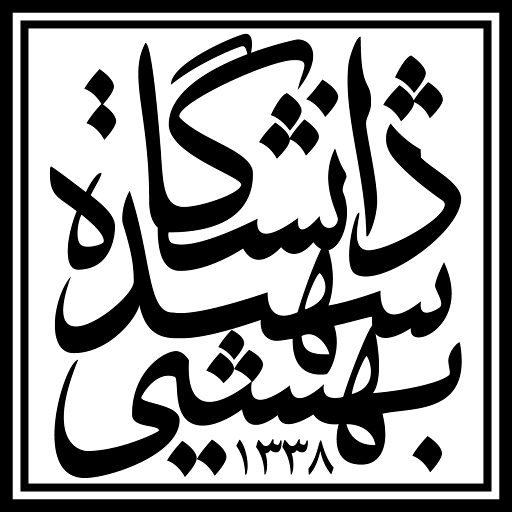
\includegraphics[width=0.32\textwidth]{logo.png}\par\vspace{1cm}

    {\Huge\bfseries Assignment Report - HW3\par}
    \vspace{0.5cm}
    {\LARGE Data Mining (Graduate Level)\par}
    \vspace{0.3cm}
    {\Large Spring 2026\par}
    \vspace{1.3cm}

    {\Large\bfseries Practical Project: American Sign Language\par}
    \vspace{1.8cm}

    \begin{tabular}{rl}
        Student Name: & Ehsan Shahbazi \\
        \\[-0.2cm]
        Student ID: & 404422100 \\
        \\[-0.2cm]
        Instructor: & Dr. Farahani \\
        \\[-0.2cm]
        Submission Date: & 27 May 2026 \\
    \end{tabular}

    \vfill
    {Department of Computer Science / Data Science\par}
\end{titlepage}

\tableofcontents
\newpage

\section{Analytical Questions}

\subsection{Q1. Transposed Convolution and Checkerboard Artifacts}

\qtext{The transposed convolution (sometimes called deconvolution) is commonly used in generative models for upsampling. Explain mathematically how overlapping kernel placements during transposed convolution can lead to ``checkerboard artifacts'' in the output. Why does a combination of nearest-neighbor upsampling followed by a standard convolution often produce visually superior results? Provide mathematical intuition.}

\ansstart
In transposed convolution, one input value is spread to many output positions by the kernel. If the stride is bigger than 1, these kernel copies do not cover the output in a perfectly even way. Some output pixels get more overlap, and some get less overlap.

In a simple 1D form, the output can be written as
\[
y[n] = \sum_m x[m]\,w[n-ms].
\]
The important part is that the number of terms inside this sum is not the same for every output location \(n\). So some places get more contributions than others.

In 2D, this uneven overlap happens in both directions. Because of that, the output can get a repeating bright-dark pattern. That is why checkerboard artifacts appear.

Nearest-neighbor upsampling followed by a normal convolution is usually cleaner. First, the image is enlarged in a uniform way. After that, a standard convolution slides over the image evenly:
\[
z = \text{Upsample}(x), \qquad
y[i,j] = \sum_{u,v} w[u,v]\,z[i-u,j-v].
\]
So every location is treated more consistently. That is why the result often looks smoother and more natural.
\ansend

\clearpage

\subsection{Q2. Equivariance Beyond Translation}

\qtext{Standard convolution is equivariant to translation, but not to other transformations like rotation or scaling. Suppose you want to build a network equivariant to 90-degree rotations. Describe how you could constrain the convolutional filters to achieve this property. What is the trade-off in terms of the number of learnable parameters compared to a standard convolution?}

\ansstart
To make the network equivariant to 90-degree rotations, I can learn one basic filter and then use its rotated copies. So if the base filter is \(w\), I also use
\[
R_{90}(w),\; R_{180}(w),\; R_{270}(w).
\]

Then I convolve the input with all of them. If the input rotates by 90 degrees, the outputs also rotate or switch channels in a predictable way. That is the main idea of equivariance.

The good part is that I do not need to learn four completely different filters. I only learn one filter and generate the other three by rotation. This is called weight sharing.

So compared to a normal convolution, the number of independent learnable parameters is smaller. The trade-off is that the model becomes more restricted. It gets better at handling rotations, but it has less freedom than a standard convolution that learns every filter separately.
\ansend

\clearpage

\subsection{Q3. Dilated Convolution and the Gridding Effect}

\qtext{Dilated (\`a trous) convolutions allow exponential expansion of the receptive field without losing resolution. However, stacking multiple dilated convolutions with the same dilation rate can cause the ``gridding'' problem. Explain mathematically what causes gridding by analyzing which input pixels contribute to a given output pixel. How does the hybrid dilation rate design (e.g., rates [1, 2, 3] in a stack) mitigate this issue?}

\ansstart
For a 1D dilated convolution with dilation \(d\), the output is
\[
y[n] = \sum_{t=0}^{k-1} w[t]\,x[n-dt].
\]
This means the filter does not read every nearby input value. It jumps with step size \(d\).

If I stack two layers with the same dilation, the gaps stay in the same pattern. Then the final output depends only on some spaced-apart input positions. Many positions in between do not affect the output at all. In 2D, these missed positions form a grid-like pattern, so this is called the gridding effect.

Hybrid dilation helps because the gaps do not stay aligned. For example, if the dilation rates are \([1,2,3]\), one layer looks at dense local information, another looks a bit farther, and the next looks even farther. Their sampling patterns mix together, so fewer input positions are ignored.

So the main idea is simple: same dilation repeated creates repeated holes, but mixed dilation rates fill more of those holes.
\ansend

\clearpage

\subsection{Q4. Receptive Field vs. Effective Receptive Field}

\qtext{While the theoretical receptive field can be calculated precisely, the effective receptive field---where the influence is concentrated---behaves differently. Explain why the effective receptive field in a randomly initialized CNN follows a Gaussian-like distribution rather than a uniform one. How does this distribution change after training, and why might this matter for tasks requiring long-range spatial dependencies?}

\ansstart
The theoretical receptive field tells us which input region can affect one output unit. But inside that region, not all pixels matter equally.

In a deep CNN, center pixels usually have more paths to the output than edge pixels. Because many paths get added together, the influence becomes strongest near the center and weaker as we move away. That shape looks more like a Gaussian than a flat uniform block.

So even if the theoretical receptive field is large, the model often uses the middle part much more than the outer part.

After training, this shape can change. The network can learn to pay more attention to useful distant regions, or it can stay very centered if local information is enough. This matters for tasks that need long-range context, like segmentation or scene understanding. If the effective receptive field stays too narrow, the model may miss important far-away information.
\ansend

\clearpage

\subsection{Q5. 1 \texorpdfstring{$\times$}{x} 1 Convolutions as Dimensionality Reduction}

\qtext{A 1 \(\times\) 1 convolution is essentially a fully connected layer applied independently to each spatial position. In the Inception architecture, 1 \(\times\) 1 convolutions are used as ``bottleneck'' layers before expensive 3 \(\times\) 3 and 5 \(\times\) 5 convolutions. Derive the reduction in computation (multiply-add operations) for a bottleneck design vs. applying a large kernel directly, given an input with \(M\) channels and bottleneck size \(B\). Why is this form of dimensionality reduction particularly well-suited to CNNs compared to PCA applied channel-wise?}

\ansstart
Suppose I want a \(k \times k\) convolution with \(M\) input channels and \(N\) output channels.

Without a bottleneck, the cost at one spatial location is
\[
C_{\text{direct}} = k^2MN.
\]

If I first use a \(1 \times 1\) convolution to reduce the channels from \(M\) to \(B\), then the cost becomes
\[
C_{\text{bottleneck}} = MB + k^2BN.
\]

If \(B\) is much smaller than \(M\), then this is much cheaper than \(k^2MN\). So the bottleneck saves computation and also reduces parameters.

This works well in CNNs because the \(1 \times 1\) layer is learned together with the whole network and keeps the spatial structure of the feature map. PCA is different. PCA is a fixed linear projection and usually is not learned end-to-end for the task. Also, PCA channel-wise does not fit naturally into the local convolution pipeline as nicely as a learned \(1 \times 1\) convolution.
\ansend

\clearpage

\subsection{Q6. Depthwise Separable Convolution and the Decoupling Assumption}

\qtext{Depthwise separable convolution factorizes a standard convolution into a depthwise spatial convolution followed by a pointwise 1 \(\times\) 1 convolution. This design implicitly assumes that spatial correlation and cross-channel correlation can be decoupled. Is this assumption always valid? Provide a counterexample scenario where this decoupling would significantly harm representational capacity. How does the MobileNet-v2 inverted residual structure partially address this limitation?}

\ansstart
No, this assumption is not always valid. Depthwise separable convolution works well in many cases, but sometimes spatial patterns and channel interactions are tightly connected and should be learned together.

A simple counterexample is when a useful pattern depends on a special combination of channels at the same time and also on their local arrangement. For example, imagine one feature only appears when channel 1 has a vertical edge and channel 2 has a horizontal edge at the same place. A standard convolution can mix channels and space together in one step. A depthwise separable layer first looks at each channel alone, so it may lose part of that joint pattern.

MobileNet-v2 helps with this problem using the inverted residual block. First it expands the number of channels with a \(1 \times 1\) convolution, then applies depthwise convolution, and then compresses again. This gives the network a larger feature space before the cheap depthwise step, so it has more room to represent useful channel combinations.

So it does not fully remove the limitation, but it makes the limitation less harmful.
\ansend

\clearpage

\subsection{Q7. Global Average Pooling as a Structural Regularizer}

\qtext{Modern CNNs often replace fully connected layers at the end of the network with Global Average Pooling (GAP), followed by a single softmax layer. Argue why GAP acts as a structural regularizer that is fundamentally different from dropout or weight decay. In particular, how does GAP enforce correspondence between feature maps and categories, and why is this correspondence more interpretable?}

\ansstart
Global Average Pooling is a structural regularizer because it changes the shape of the model itself, not just the training penalty. Dropout randomly removes activations during training, and weight decay pushes weights to stay small. GAP does something different: it forces each feature map to be summarized by one average value.

If one feature map becomes strong, its average becomes large. Then the final classifier uses that average to help predict a class. So feature maps are pushed to behave like class-related detectors instead of sending many location-specific values into a big fully connected layer.

This makes the model more interpretable because I can more easily say: this feature map responds strongly to patterns related to this class. With a big fully connected layer, the last decision is spread across many weights and is harder to read.

So GAP reduces parameters, reduces overfitting, and also gives a cleaner connection between learned feature maps and output classes.
\ansend

\clearpage

\subsection{Q8. Adversarial Patches and the Local Nature of Convolutions}

\qtext{An adversarial patch---a small, localized perturbation---can cause a CNN to misclassify an entire image with high confidence, even when the patch covers only a tiny fraction of the input. Explain, using the mechanics of convolutions and receptive fields, why CNNs are particularly vulnerable to this type of attack. How do architectural choices like large kernels or dilated convolutions influence this vulnerability?}

\ansstart
CNNs are built from local filters. A small patch can strongly activate some local filters if it contains a pattern the network finds very important. Once those activations become large, they keep getting combined in deeper layers. So a small local change can spread its effect through bigger and bigger receptive fields until it affects the final decision for the whole image.

This is one reason adversarial patches can work so well. The patch does not need to change the full image. It only needs to create a strong local signal that the network trusts too much.

Large kernels or dilated convolutions can make this effect spread even faster, because one local patch can influence a wider region in fewer layers. On the other hand, they can also give more context in some models. So they do not automatically solve the problem. In some cases they can even make the patch affect more of the network more quickly.

The core issue is that local evidence can get amplified a lot inside a CNN.
\ansend

\clearpage

\subsection{Q9. Strided Convolution vs. Max-Pooling for Downsampling}

\qtext{Both strided convolution and max-pooling can be used to reduce spatial dimensions. Compare them in terms of learnable parameters, gradient flow, and the type of information they discard. Under what circumstances might a strided convolution fail to learn an effective downsampling operation that max-pooling achieves trivially? Could a learned combination (e.g., max-pooling followed by a 1 \(\times\) 1 convolution) offer the best of both worlds?}

\ansstart
Max-pooling has no learnable parameters. It simply keeps the strongest value in each local region. Strided convolution has learnable weights, so it can learn a smarter downsampling rule, but it also has to learn that rule from data.

They also discard information in different ways. Max-pooling keeps the strongest activation and throws away the rest. Strided convolution mixes values with learned weights and then samples at larger steps, so it can smooth, combine, or suppress information depending on training.

Sometimes strided convolution may fail when the model does not learn a good downsampling filter. For example, if training is weak or data is limited, it may not learn to preserve the strongest local feature as cleanly as max-pooling does automatically. Max-pooling gets that behavior for free.

Yes, a combination can be a good idea. Max-pooling can give stable downsampling, and then a \(1 \times 1\) convolution can learn how to mix channels after that. This can give some of the simplicity of pooling and some of the flexibility of learned layers.
\ansend

\clearpage

\section{Practical Project}

\subsection{2.1 Dataset: American Sign Language}

\qtext{Describe the dataset and explain the split that was used.}

\ansstart
This project uses an American Sign Language image dataset. Each image shows one hand sign for an English letter, and each row in the annotation CSV gives the image name, bounding box coordinates, and the class label. The bounding box tells me where the hand is, so I used it as the main feature extraction step before training.

The dataset was already split into three folders: `train`, `valid`, and `test`. I kept this split exactly as it was given, so my work stays reproducible and fair. I did not move images between splits.

From the notebook, the dataset has 1,728 images in total. The train split has 1,512 images, the validation split has 144 images, and the test split has 72 images. The train and validation splits contain all 26 letters from A to Z, but the test split contains only 24 classes. The letters `E` and `L` do not appear in the test set, so their test support is zero. This is important when reading the classification report later.
\ansend

\begin{table}[H]
\centering
\caption{Dataset size by split}
\begin{tabular}{lcc}
\toprule
Split & Number of images & Number of classes \\
\midrule
Train & 1512 & 26 \\
Validation & 144 & 26 \\
Test & 72 & 24 \\
\bottomrule
\end{tabular}
\end{table}

\qtext{What does the class distribution look like?}

\ansstart
The training set is not perfectly balanced, but it is still usable. In the train split, the smallest class has 39 images and the largest class has 78 images. In the validation split, counts go from 1 to 9 images, and in the test split they go from 1 to 5 images. So the validation and test sets are much smaller and more sensitive to small changes.

This matters because classes with fewer examples can be harder for the model, and small test support can make per-class scores look unstable. For example, if a class has only one test image, one correct or wrong prediction changes its score a lot.
\ansend

\begin{figure}[H]
    \centering
    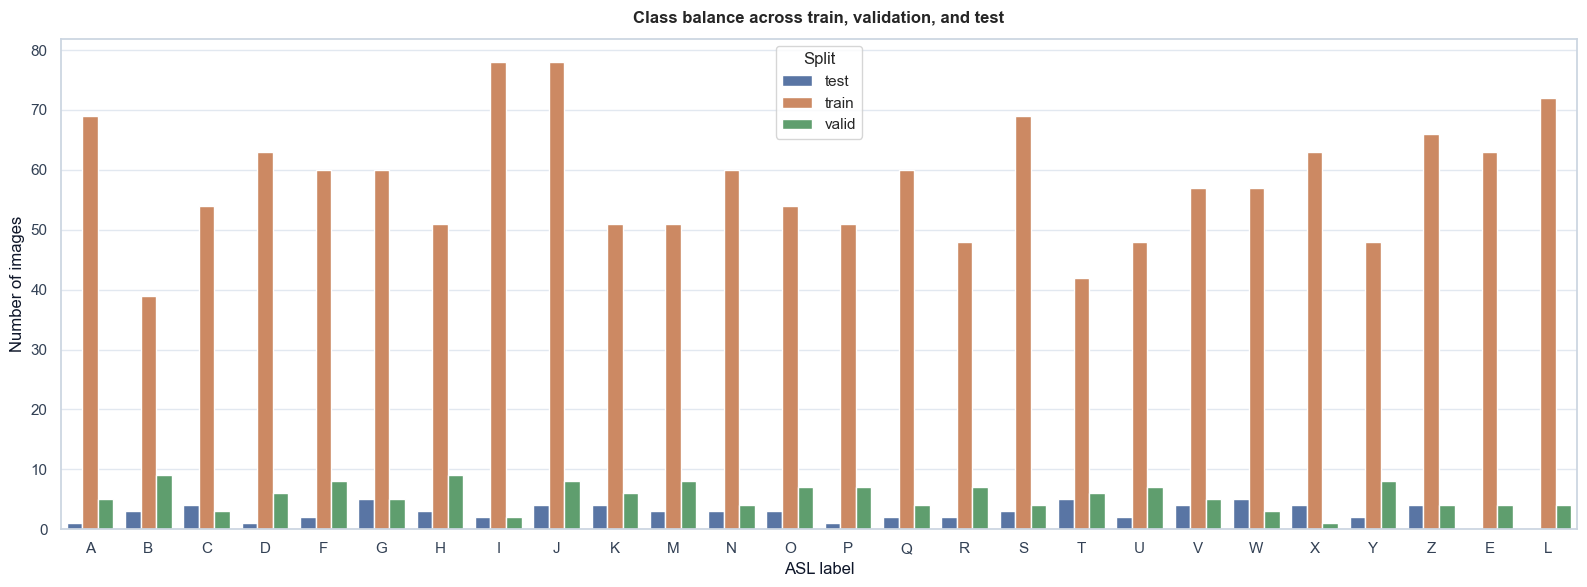
\includegraphics[width=0.95\textwidth]{report_figures/cell_10_0.png}
    \caption{Class balance across train, validation, and test splits.}
\end{figure}

\subsection{2.2 Exploratory Data Analysis (EDA) and Data Preprocessing}

\subsubsection{Dataset and bounding box analysis}

\qtext{What did the EDA show about image size, bounding boxes, and data quality?}

\ansstart
The images are close in size, around 372 to 416 pixels on each side, so the raw data is already fairly consistent. I then checked the hand bounding boxes because the whole preprocessing pipeline depends on them.

The average bounding box width is about 222.60 pixels and the average height is about 210.69 pixels. The average hand area covers about 31.6\% of the full image area. The median area ratio is about 28.6\%, which means the hand usually takes a meaningful part of the image, but it does not fill the whole image.

I also ran simple quality checks. There were no missing files, no broken coordinate order, no negative coordinates, and no boxes that went outside the image border. So the annotations looked clean and safe to use.
\ansend

\begin{table}[H]
\centering
\caption{Bounding box summary from the notebook}
\begin{tabular}{lrrrr}
\toprule
Measure & Mean & Min & Median & Max \\
\midrule
BBox width & 222.60 & 74 & 217 & 404 \\
BBox height & 210.69 & 59 & 203 & 414 \\
BBox area ratio & 0.316 & 0.036 & 0.286 & 0.966 \\
\bottomrule
\end{tabular}
\end{table}

\begin{table}[H]
\centering
\caption{Data quality check summary}
\begin{tabular}{lc}
\toprule
Check & Count \\
\midrule
Missing image file & 0 \\
Invalid x order & 0 \\
Invalid y order & 0 \\
Negative coordinate & 0 \\
X outside image border & 0 \\
Y outside image border & 0 \\
\bottomrule
\end{tabular}
\end{table}

\begin{figure}[H]
    \centering
    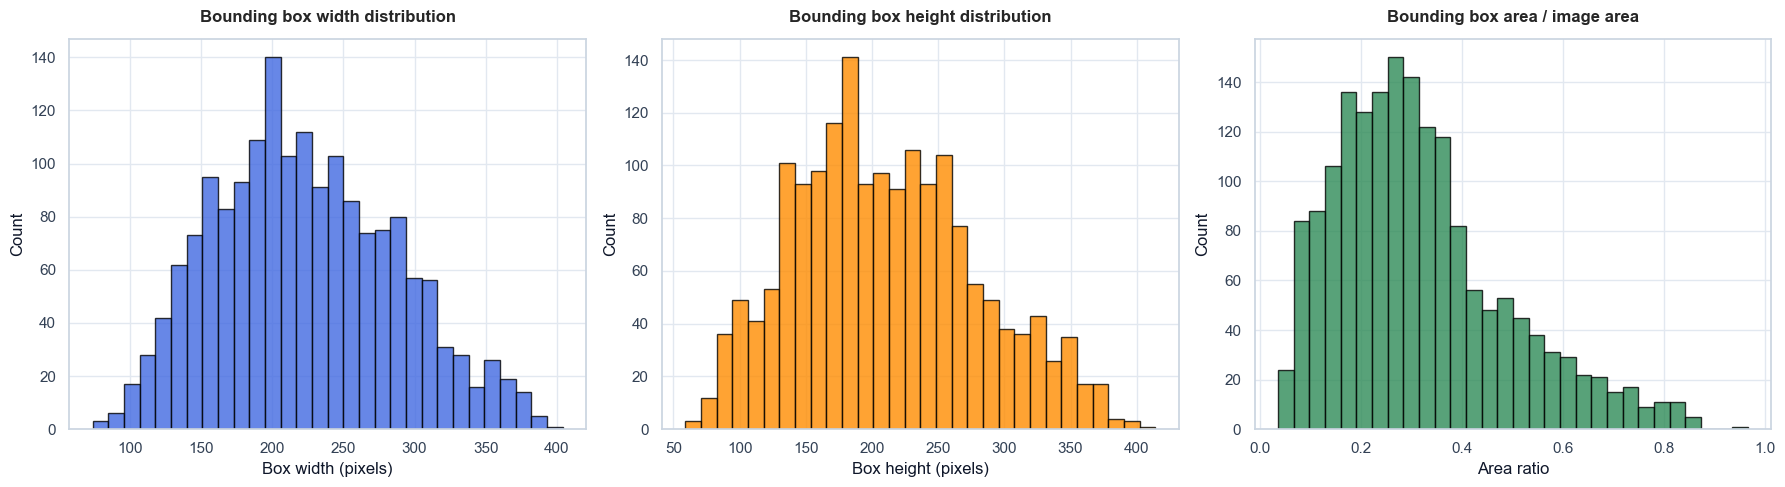
\includegraphics[width=0.95\textwidth]{report_figures/cell_15_0.png}
    \caption{Bounding box width, height, and area ratio distributions.}
\end{figure}

\begin{figure}[H]
    \centering
    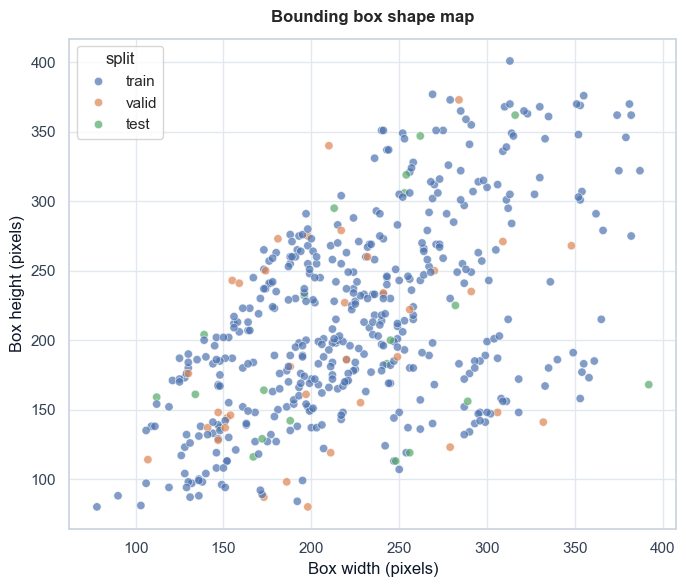
\includegraphics[width=0.55\textwidth]{report_figures/cell_16_0.png}
    \caption{Bounding box shape map using width and height.}
\end{figure}

\begin{figure}[H]
    \centering
    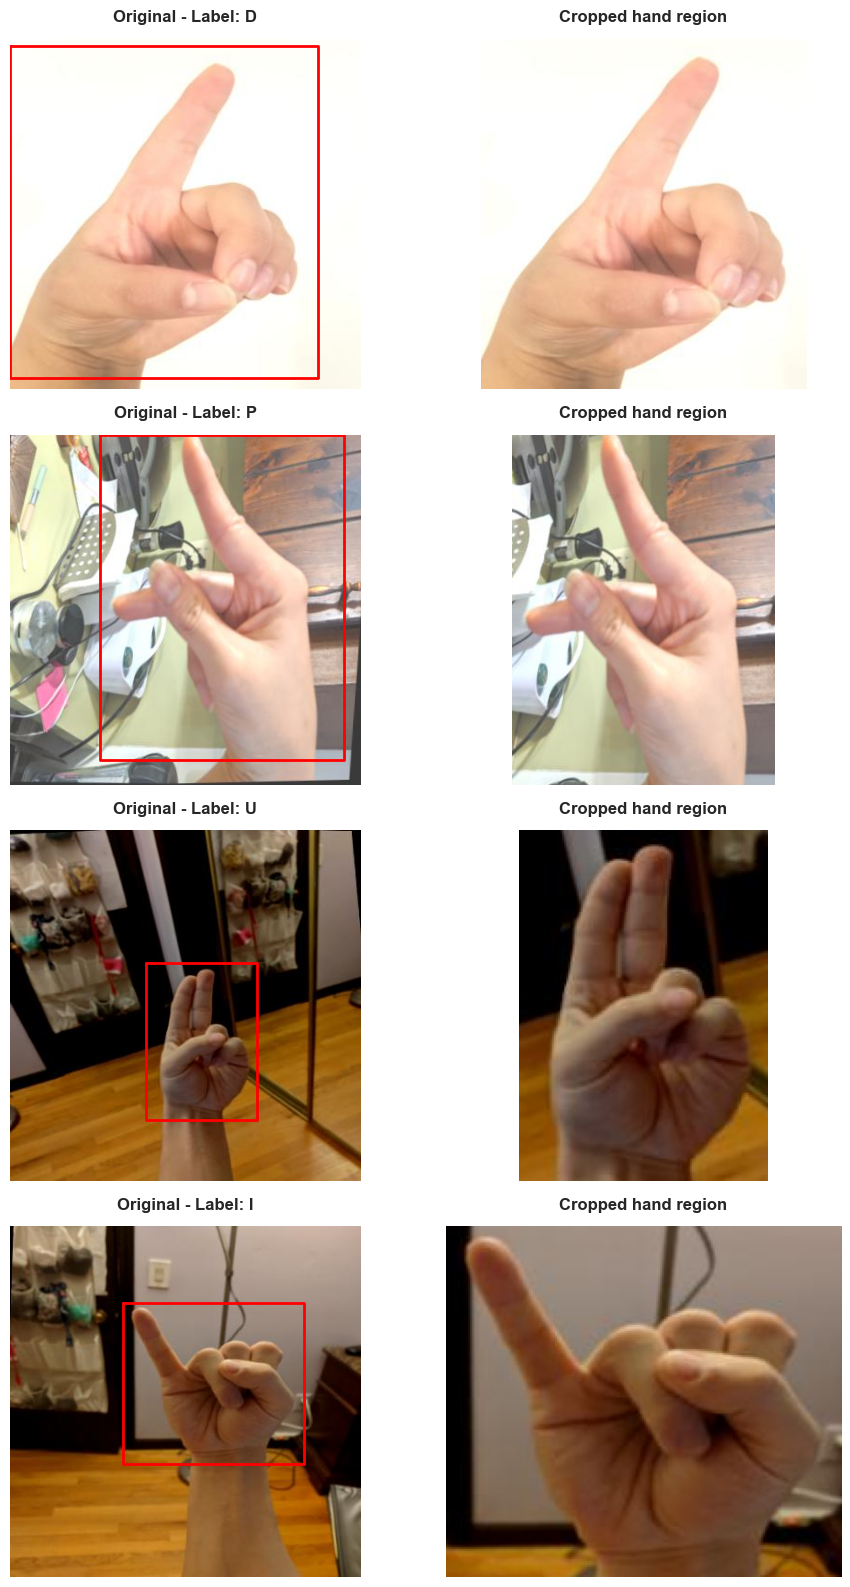
\includegraphics[width=0.8\textwidth]{report_figures/cell_20_0.png}
    \caption{Examples of original images with their bounding boxes.}
\end{figure}

\qtext{What preprocessing pipeline was used, and why?}

\ansstart
I used one clear pipeline for all splits:
\begin{enumerate}[leftmargin=1.2cm]
    \item load the image,
    \item crop the hand using the given bounding box,
    \item resize the cropped image to a fixed size,
    \item convert it to an array,
    \item normalize the pixel values.
\end{enumerate}

The same core steps were used for train, validation, and test. This follows the assignment rule that feature extraction must be consistent across all splits.
\ansend

\subsubsection{Cropping}

\qtext{How was cropping done?}

\ansstart
For each image, I cropped the region inside the bounding box. This step removes a lot of background and keeps the hand as the main object. I also clamped the box values to stay inside the image border, just to make the pipeline safe even if a box is close to the edge.

Cropping is important here because the task is hand sign recognition, not background recognition. By using only the hand region, the model gets a cleaner input.
\ansend

\subsubsection{Resizing}

\qtext{What fixed size was used, and why?}

\ansstart
I resized all cropped images to \textbf{128 \(\times\) 128}. I chose this size because it is a good middle point. A size like 64 \(\times\) 64 is faster, but it may lose finger details. A size like 224 \(\times\) 224 keeps more detail, but it is heavier and slower for my hardware. So 128 \(\times\) 128 gave me a good balance between detail and speed.
\ansend

\subsubsection{Normalization}

\qtext{What normalization was used, and why?}

\ansstart
I normalized pixel values to the range \([0,1]\) by dividing by 255. This choice is simple, common, and easy to explain. It also keeps training stable because all inputs stay on the same scale.

After preprocessing, the notebook confirmed that the train, validation, and test arrays had shapes `(1512, 128, 128, 3)`, `(144, 128, 128, 3)`, and `(72, 128, 128, 3)`, and the pixel range was from 0.0 to 1.0.
\ansend

\subsubsection{Data augmentation}

\qtext{What augmentation was used, and where was it applied?}

\ansstart
Augmentation was applied \textbf{only to the training set}. I did not apply augmentation to validation or test data because that would make evaluation unfair.

In the notebook, I used several small and realistic augmentations:
\begin{itemize}[leftmargin=1.2cm]
    \item random rotation,
    \item random translation,
    \item brightness adjustment,
    \item random left-right flip,
    \item random zoom.
\end{itemize}

The main idea was to help the model handle normal variation in hand position, angle, and lighting. I kept the changes small so the hand sign still looks like the same class.
\ansend

\begin{figure}[H]
    \centering
    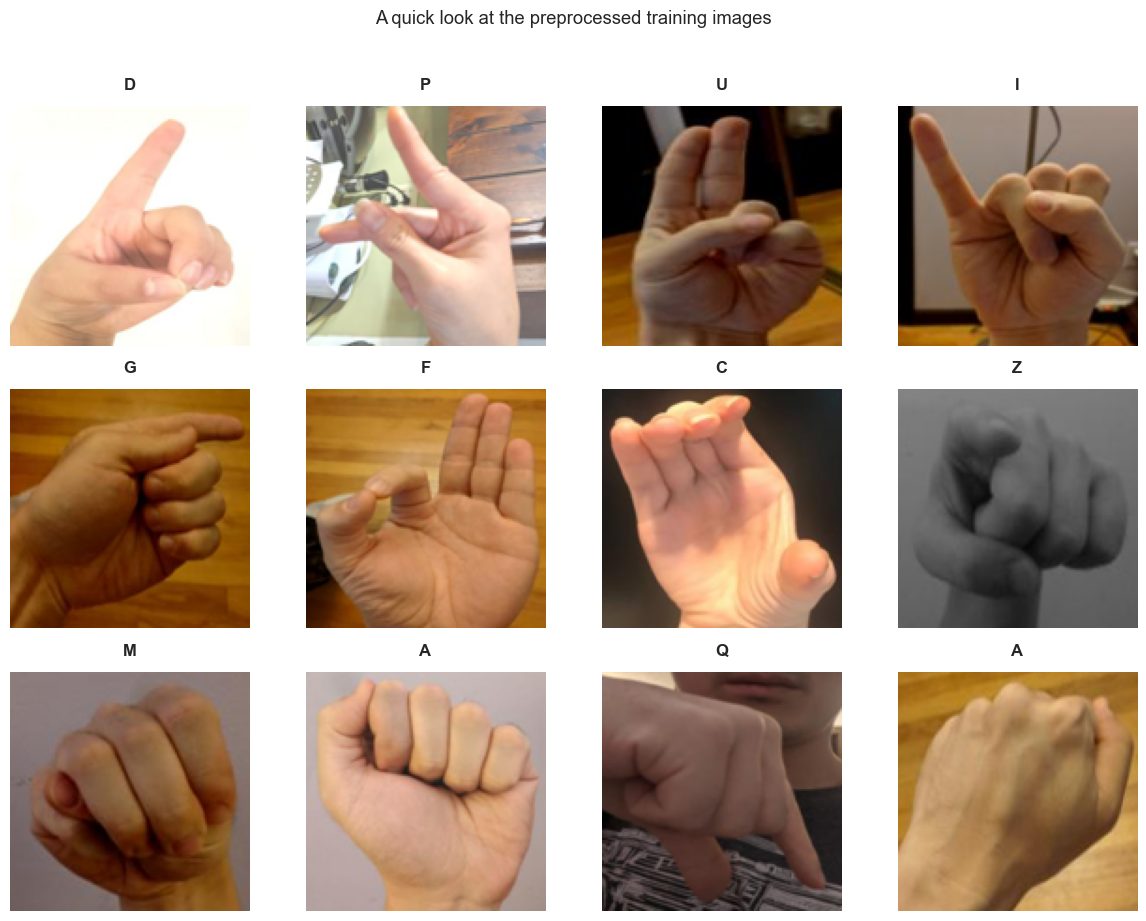
\includegraphics[width=0.78\textwidth]{report_figures/cell_27_0.png}
    \caption{Examples of preprocessed training images after crop, resize, and normalization.}
\end{figure}

\begin{figure}[H]
    \centering
    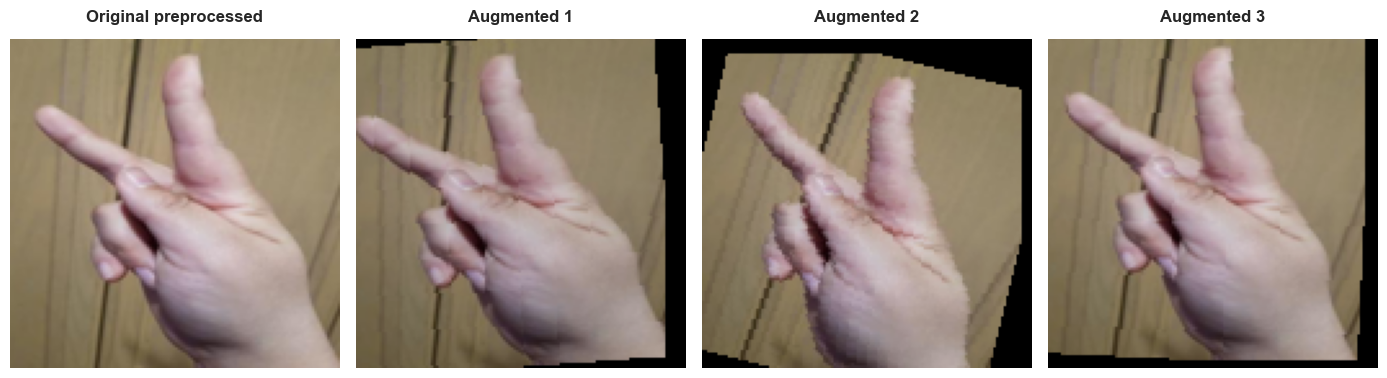
\includegraphics[width=0.95\textwidth]{report_figures/cell_28_0.png}
    \caption{One preprocessed image and three augmented versions.}
\end{figure}

\subsection{2.3 CNN Classification}

\qtext{What model and training setup were used?}

\ansstart
I used a CNN built in PyTorch. The model starts with a small stem layer, then uses residual blocks with max-pooling, and ends with adaptive average pooling and two fully connected layers. I used batch normalization and dropout to help training stay stable and reduce overfitting.

The loss function was categorical cross entropy through \texttt{CrossEntropyLoss}. The optimizer was \texttt{AdamW}. I also used class weights because the class counts were not perfectly balanced. The main training settings from the notebook were:
\begin{itemize}[leftmargin=1.2cm]
    \item batch size = 16,
    \item maximum epochs = 60 for the first main model,
    \item early stopping patience = 10,
    \item learning rate = 0.0008,
    \item weight decay = 0.0001,
    \item label smoothing = 0.05,
    \item checkpoint saving based on best validation accuracy.
\end{itemize}

The notebook ran on Apple Silicon using the `mps` device. The first main model used all 60 epochs, and the best checkpoint was saved during training.
\ansend

\begin{figure}[H]
    \centering
    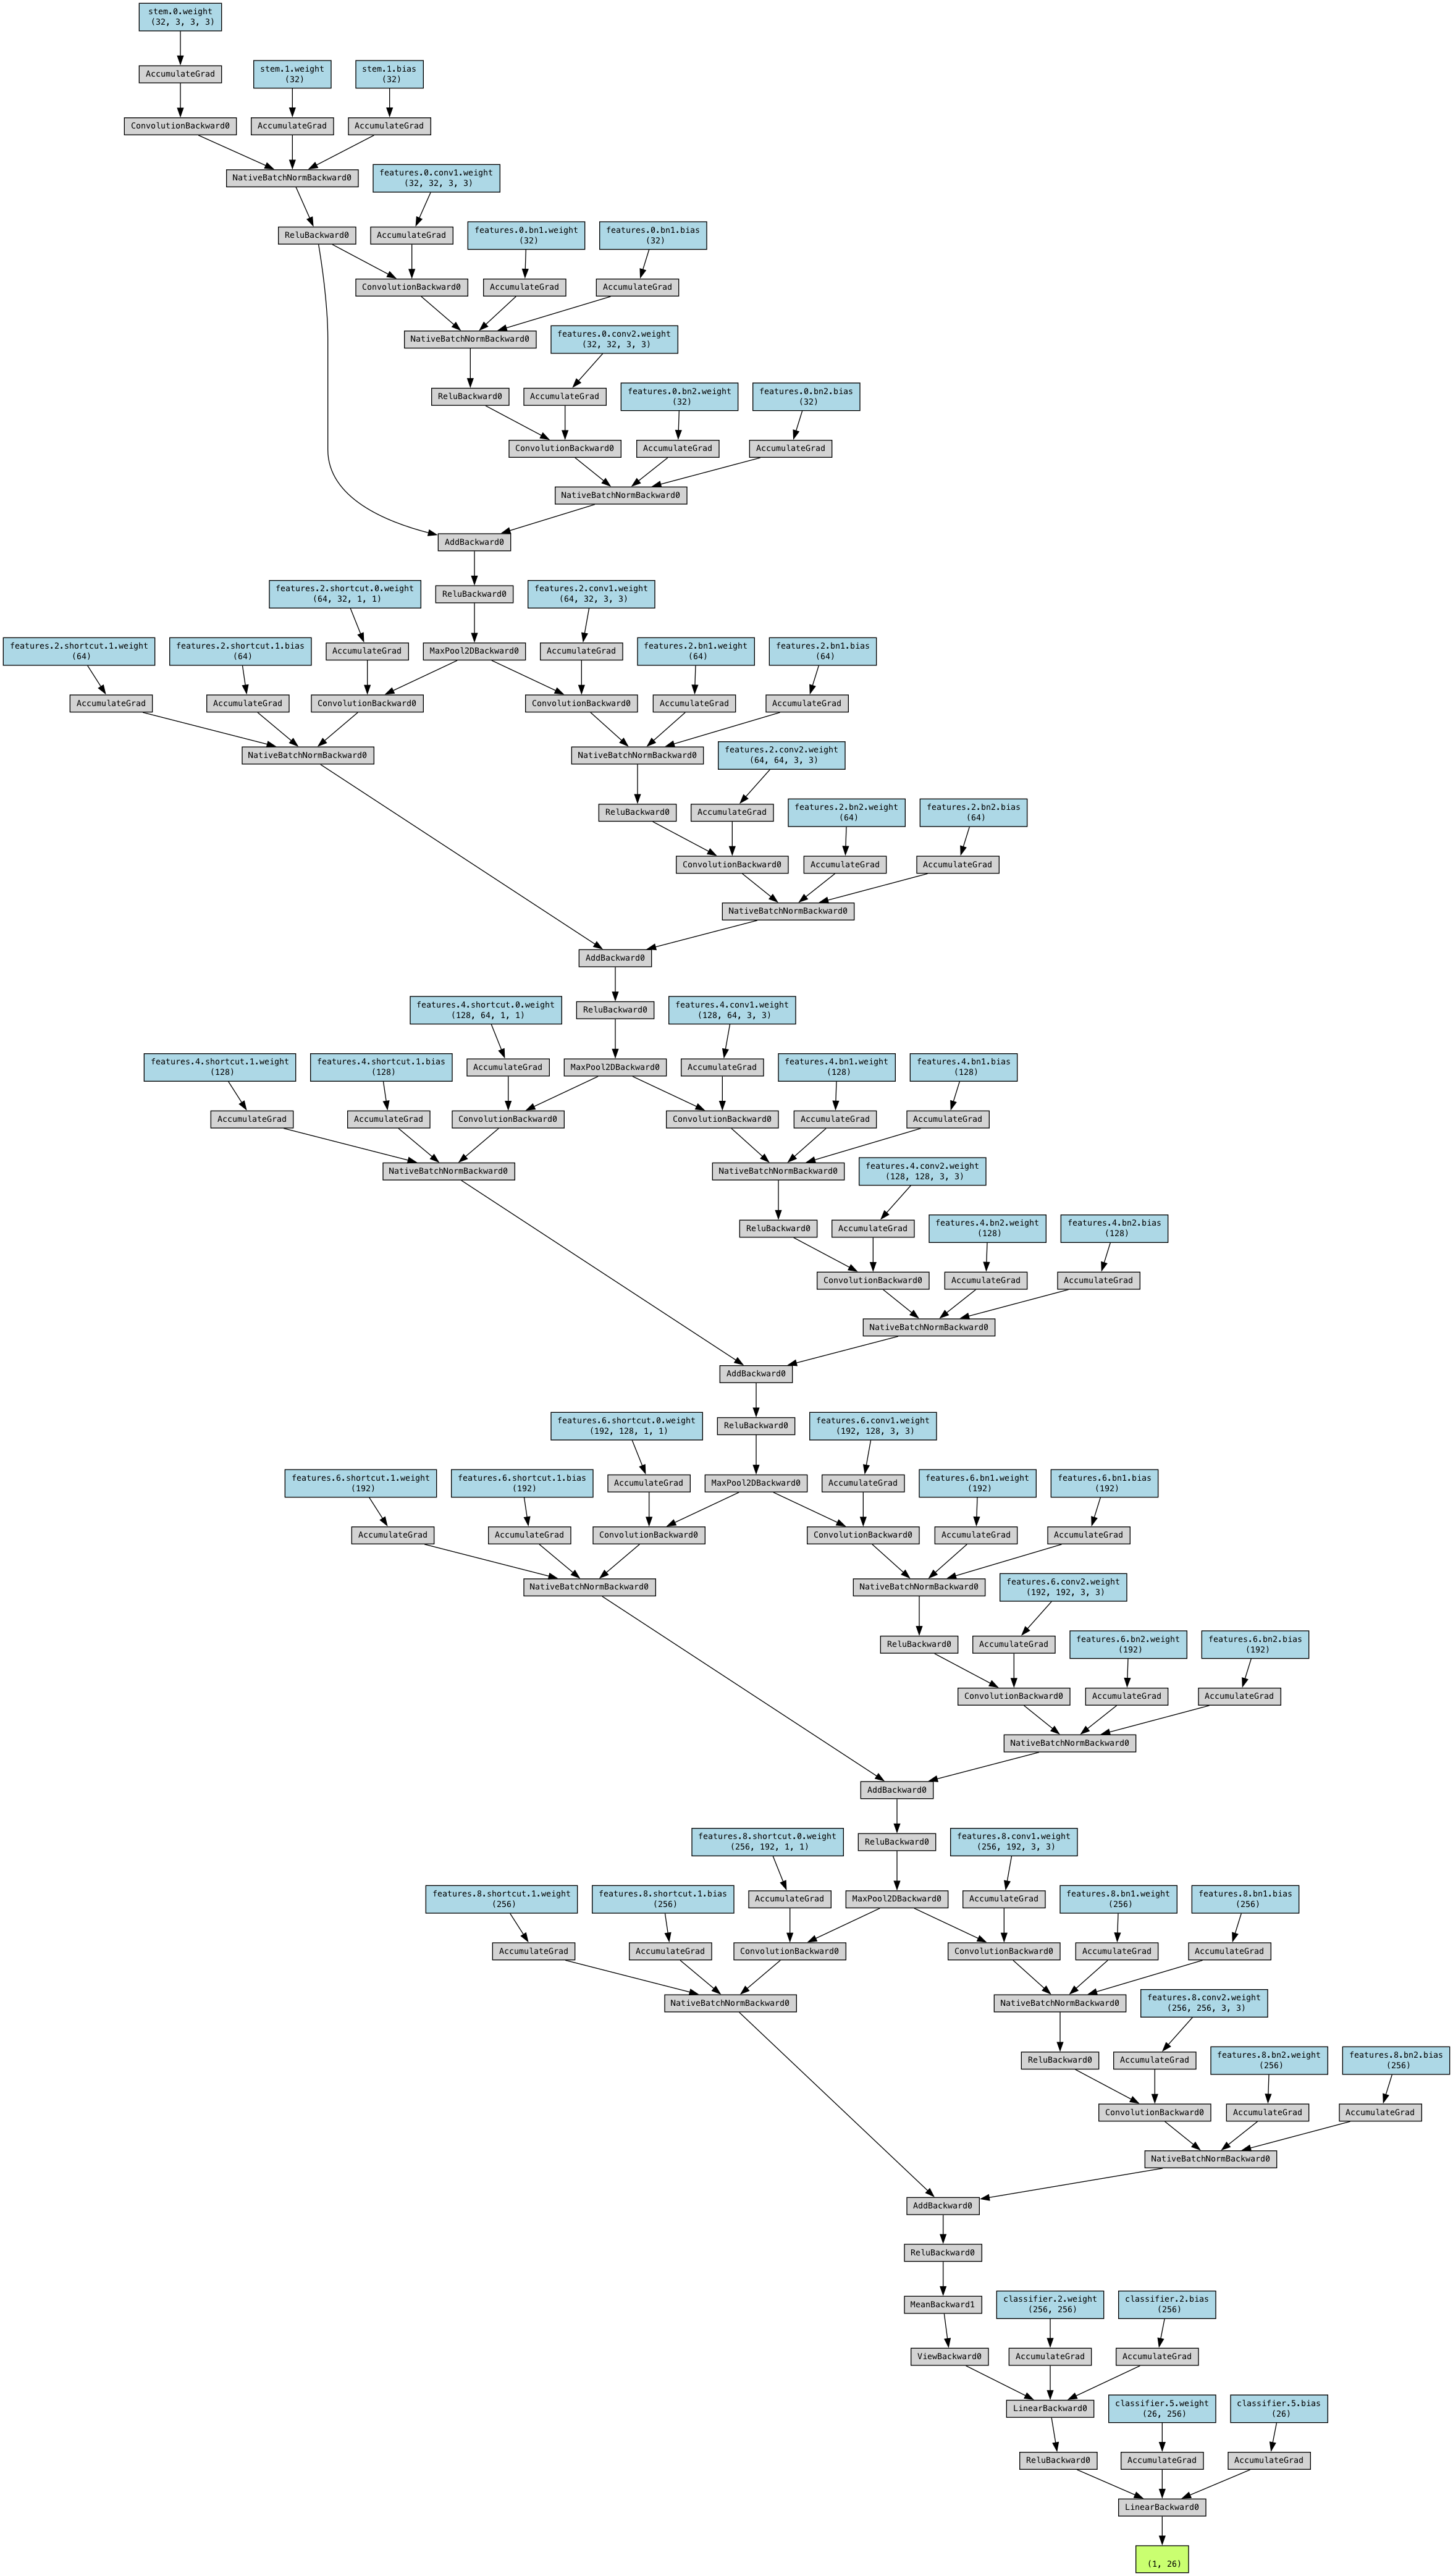
\includegraphics[width=0.78\textwidth]{asl_model_viz.png}
    \caption{Saved visualization of the CNN computation graph.}
\end{figure}

\qtext{How did training behave?}

\ansstart
The learning curves looked healthy overall. Train loss went down, validation loss also improved, and validation accuracy increased during training. This shows that the model was learning useful features from the cropped hand images.

There was still some gap between train and validation curves later in training, which is normal in image classification. That is one reason I used dropout, augmentation, and checkpoint saving.
\ansend

\begin{figure}[H]
    \centering
    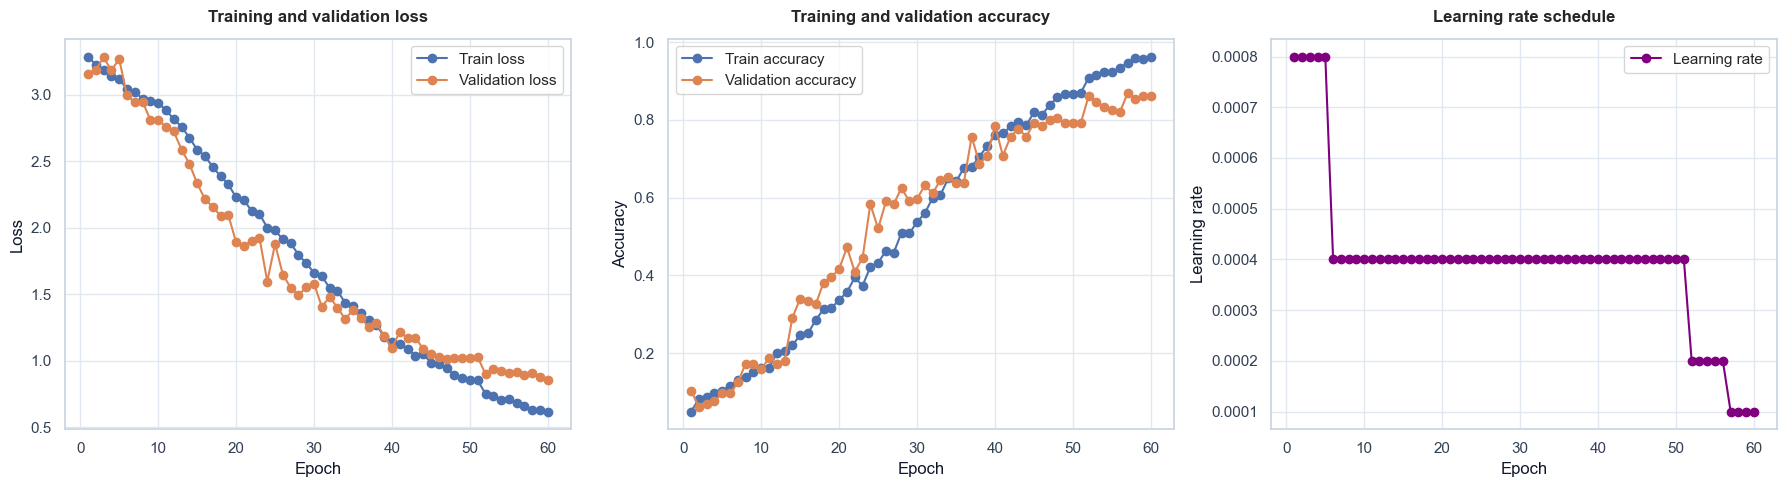
\includegraphics[width=0.97\textwidth]{report_figures/cell_48_0.png}
    \caption{Training loss, validation loss, accuracy, and learning rate curves.}
\end{figure}

\qtext{Did I try more than one setup?}

\ansstart
Yes. After the first strong model, I also tried four nearby training setups to compare results. The four versions changed batch size, learning rate, weight decay, and label smoothing. I increased the epoch limit to 100 in that search, but I kept early stopping so the model could stop when it stopped improving.

The best validation score in that search came from `model\_4\_more\_regularized`, which reached validation accuracy 0.8889. But its test accuracy was only 0.8056. Since the assignment says test accuracy is the main score, I did not choose that one as my final model.

The first main CNN gave the highest test accuracy in my notebook, so I used that model as the final model in this report.
\ansend

\begin{table}[H]
\centering
\caption{Comparison of the four extra experiment settings}
\begin{tabular}{lcccc}
\toprule
Model & Best epoch & Validation acc. & Test acc. & Macro F1 \\
\midrule
model\_4\_more\_regularized & 59 & 0.8889 & 0.8056 & 0.7246 \\
model\_2\_lower\_lr & 73 & 0.8750 & 0.7917 & 0.7136 \\
model\_1\_baseline\_plus & 84 & 0.8681 & 0.8194 & 0.7452 \\
model\_3\_larger\_batch & 74 & 0.8611 & 0.7778 & 0.6993 \\
\bottomrule
\end{tabular}
\end{table}

\begin{figure}[H]
    \centering
    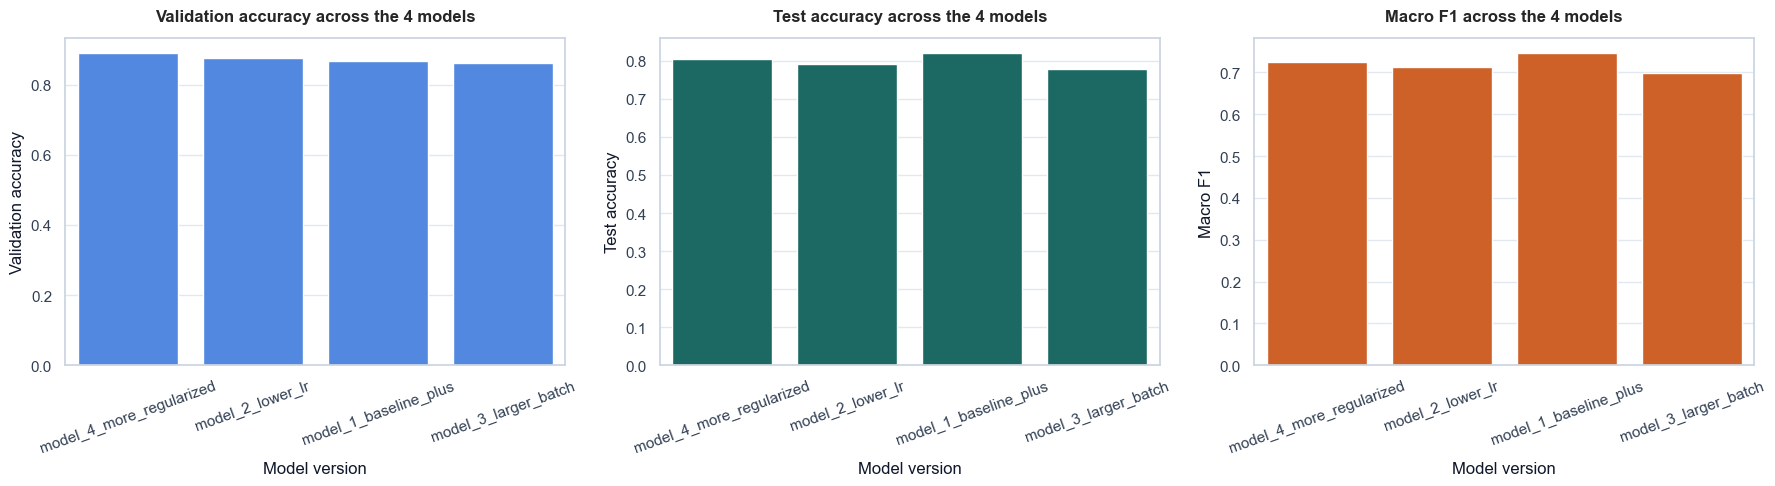
\includegraphics[width=0.97\textwidth]{report_figures/cell_98_0.png}
    \caption{Comparison of the four extra model versions.}
\end{figure}

\subsection{2.4 Model Evaluation and Comparative Analysis}

\qtext{What were the final test results for the best model by test accuracy?}

\ansstart
My final model is the first main PyTorch CNN because it gave the highest test accuracy in the notebook. Its final results were:
\begin{itemize}[leftmargin=1.2cm]
    \item validation accuracy = 0.8681,
    \item test accuracy = 0.8611,
    \item macro precision = 0.8154,
    \item macro recall = 0.7891,
    \item macro F1-score = 0.7621,
    \item weighted precision = 0.9148,
    \item weighted recall = 0.8611,
    \item weighted F1-score = 0.8535.
\end{itemize}

The weighted scores are higher than the macro scores. This tells me the model did better on classes with more effective support, while a few classes were weaker. Also, because the test set is small and misses `E` and `L`, the macro scores are affected more strongly.
\ansend

\begin{table}[H]
\centering
\caption{Final evaluation metrics for the selected model}
\begin{tabular}{lc}
\toprule
Metric & Value \\
\midrule
Validation Accuracy & 0.8681 \\
Test Accuracy & 0.8611 \\
Macro Precision & 0.8154 \\
Macro Recall & 0.7891 \\
Macro F1-Score & 0.7621 \\
Weighted Precision & 0.9148 \\
Weighted Recall & 0.8611 \\
Weighted F1-Score & 0.8535 \\
\bottomrule
\end{tabular}
\end{table}

\qtext{What does the confusion matrix show?}

\ansstart
The confusion matrix shows that many classes were predicted correctly, but a few pairs were mixed up. The notebook showed these top confusion pairs:
\begin{itemize}[leftmargin=1.2cm]
    \item F predicted as B,
    \item I predicted as D,
    \item M predicted as A,
    \item M predicted as H,
    \item O predicted as N,
    \item O predicted as Q,
    \item R predicted as X,
    \item T predicted as A,
    \item T predicted as N,
    \item V predicted as K.
\end{itemize}

Most of these errors make sense because some hand shapes look close to each other, especially when finger position changes only a little. Another reason is that some classes have very small support in the test set, so one mistake is enough to reduce the class score a lot.
\ansend

\begin{figure}[H]
    \centering
    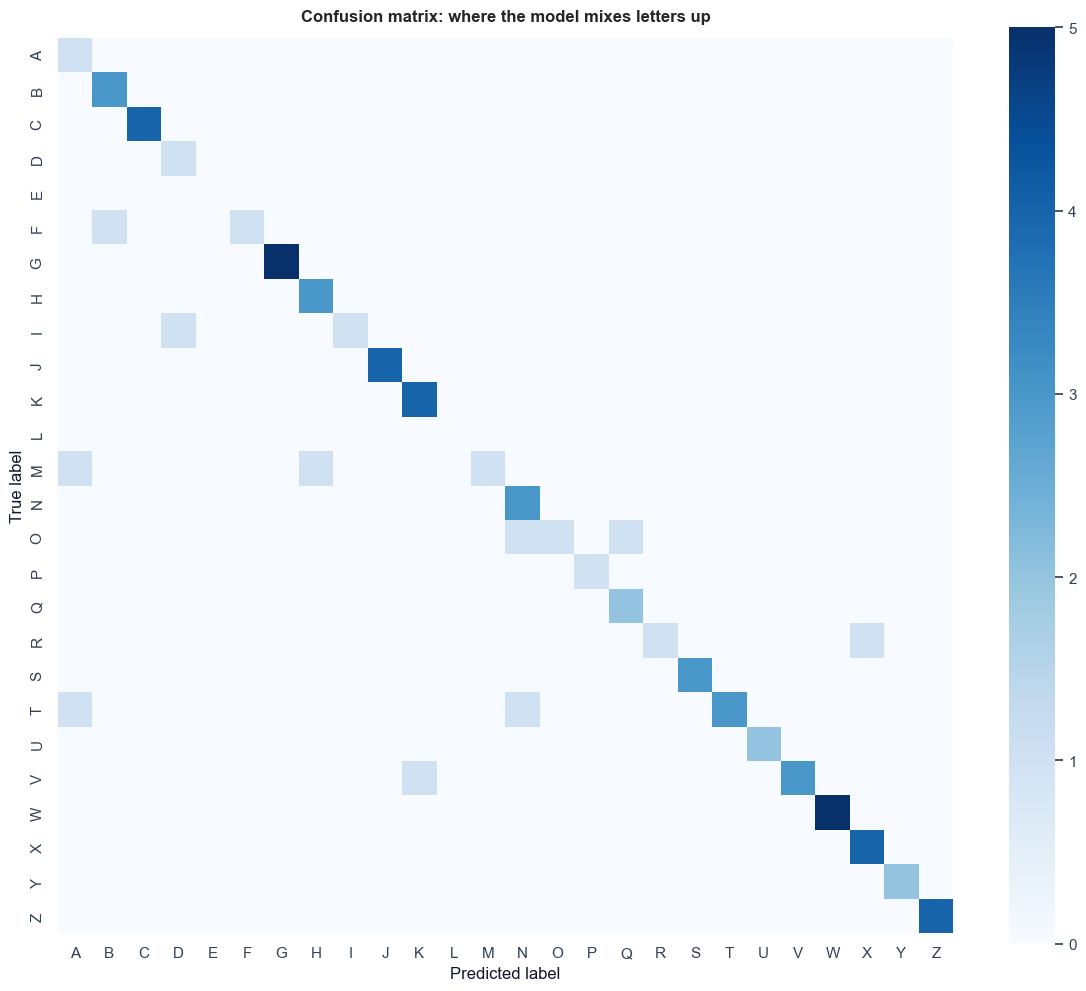
\includegraphics[width=0.82\textwidth]{report_figures/cell_55_0.png}
    \caption{Confusion matrix for the final model.}
\end{figure}

\begin{figure}[H]
    \centering
    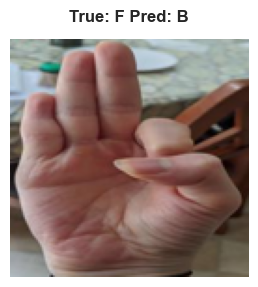
\includegraphics[width=0.42\textwidth]{report_figures/cell_75_0.png}
    \caption{Example from the top confusion pair analysis.}
\end{figure}

\qtext{Which classes were easiest and hardest?}

\ansstart
From the per-class report, strong classes included C, G, J, P, S, U, W, Y, and Z, all with very good or perfect test behavior in this split. Weaker classes included M and O, each with accuracy 0.3333, and F, I, and R, each with accuracy 0.5000. T was also harder than many others, with accuracy 0.6000.

For `E` and `L`, the test support was zero, so their zero values in the report do not mean the model failed on visible samples. It only means those classes were not present in the test set.
\ansend

\begin{figure}[H]
    \centering
    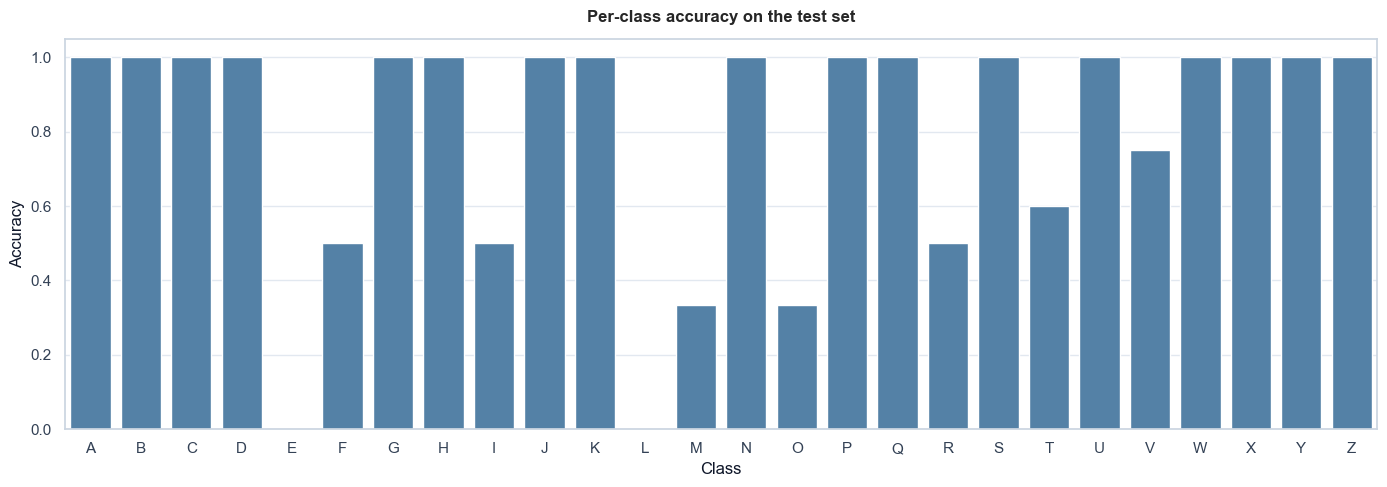
\includegraphics[width=0.9\textwidth]{report_figures/cell_72_0.png}
    \caption{Per-class accuracy on the test set.}
\end{figure}

\begin{figure}[H]
    \centering
    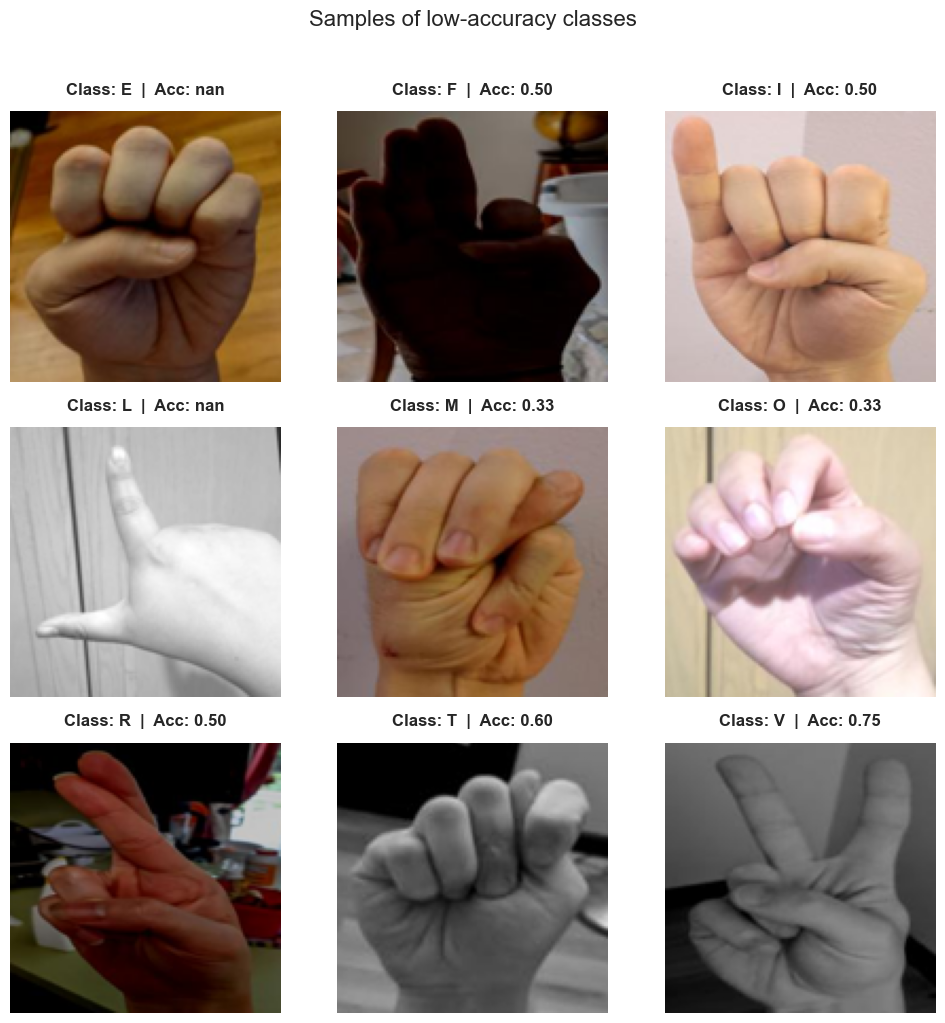
\includegraphics[width=0.78\textwidth]{report_figures/cell_73_0.png}
    \caption{Selected letters with their test accuracy values.}
\end{figure}

\qtext{What extra analysis did the notebook show?}

\ansstart
I added extra analysis so the report is not based only on one accuracy number.

First, I looked at wrong predictions directly. The misclassified sample gallery helped me see if the model mistakes looked understandable. In many cases, the wrong class had a similar hand shape.

Second, I checked model confidence. The notebook showed that correct predictions had mean confidence about 0.8505, while wrong predictions had mean confidence about 0.4568. This is a good sign because the model is usually more sure when it is correct and less sure when it is wrong.

Third, I used Grad-CAM, saliency maps, PCA, and t-SNE. These plots helped me see where the model looked and how learned features were grouped. In general, the heatmaps focused on the hand region, which supports the idea that cropping worked well and the model learned useful sign features.
\ansend

\begin{figure}[H]
    \centering
    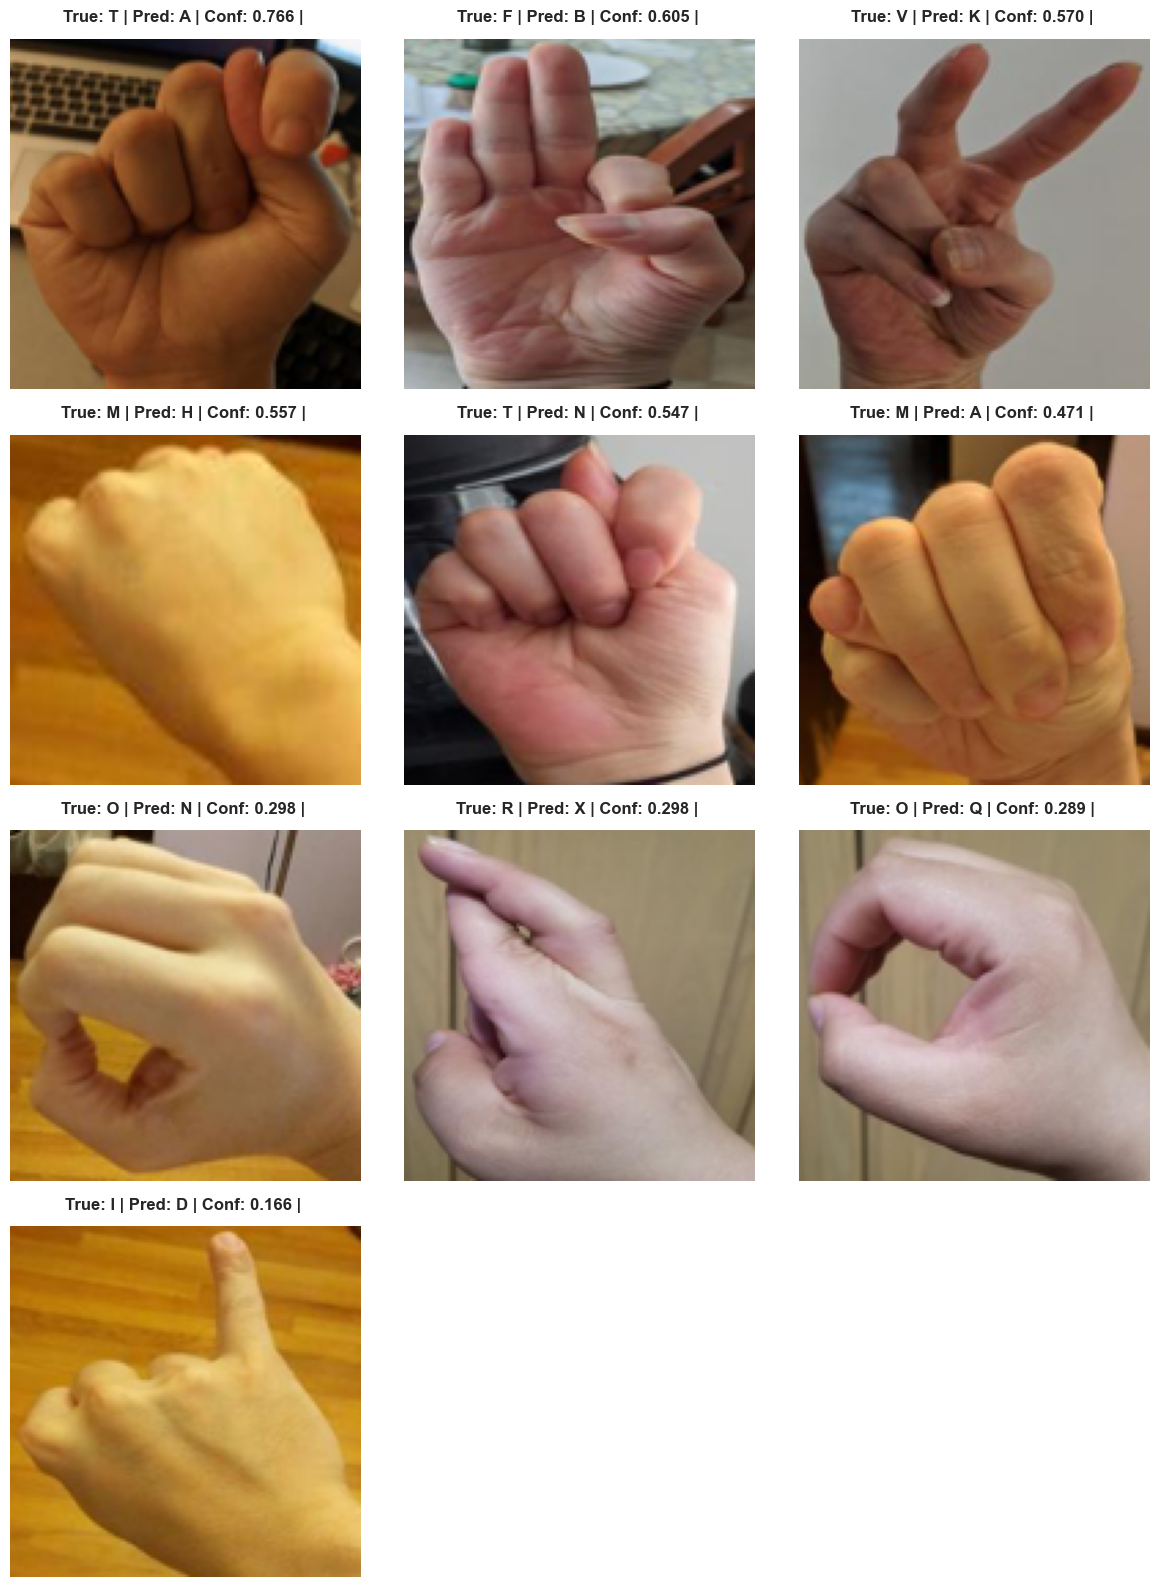
\includegraphics[width=0.82\textwidth]{report_figures/cell_68_0.png}
    \caption{Gallery of misclassified test samples.}
\end{figure}

\begin{figure}[H]
    \centering
    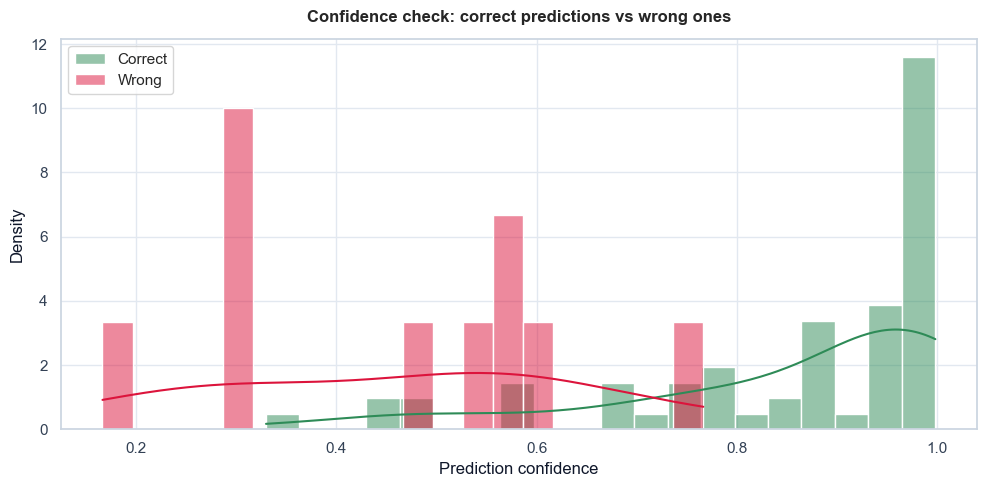
\includegraphics[width=0.78\textwidth]{report_figures/cell_70_0.png}
    \caption{Confidence distribution for correct and wrong predictions.}
\end{figure}

\begin{figure}[H]
    \centering
    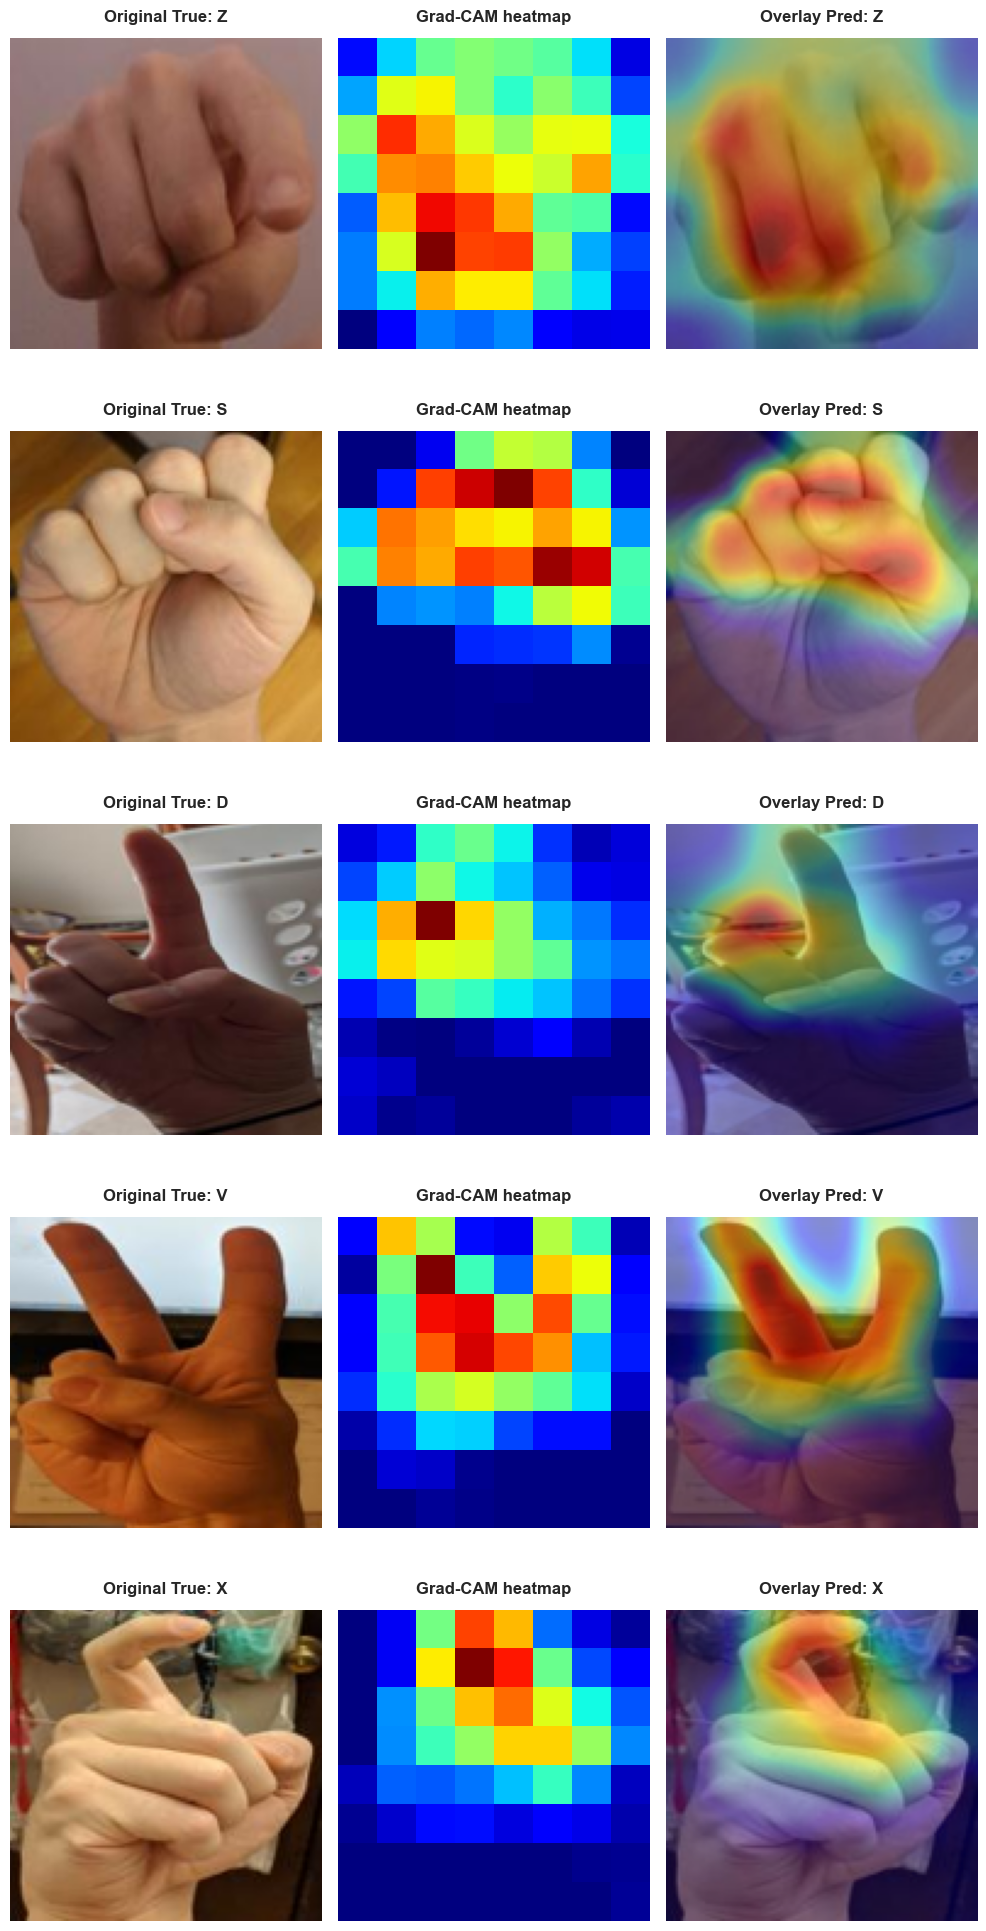
\includegraphics[width=0.82\textwidth]{report_figures/cell_78_0.png}
    \caption{Grad-CAM examples showing where the model is looking.}
\end{figure}

\begin{figure}[H]
    \centering
    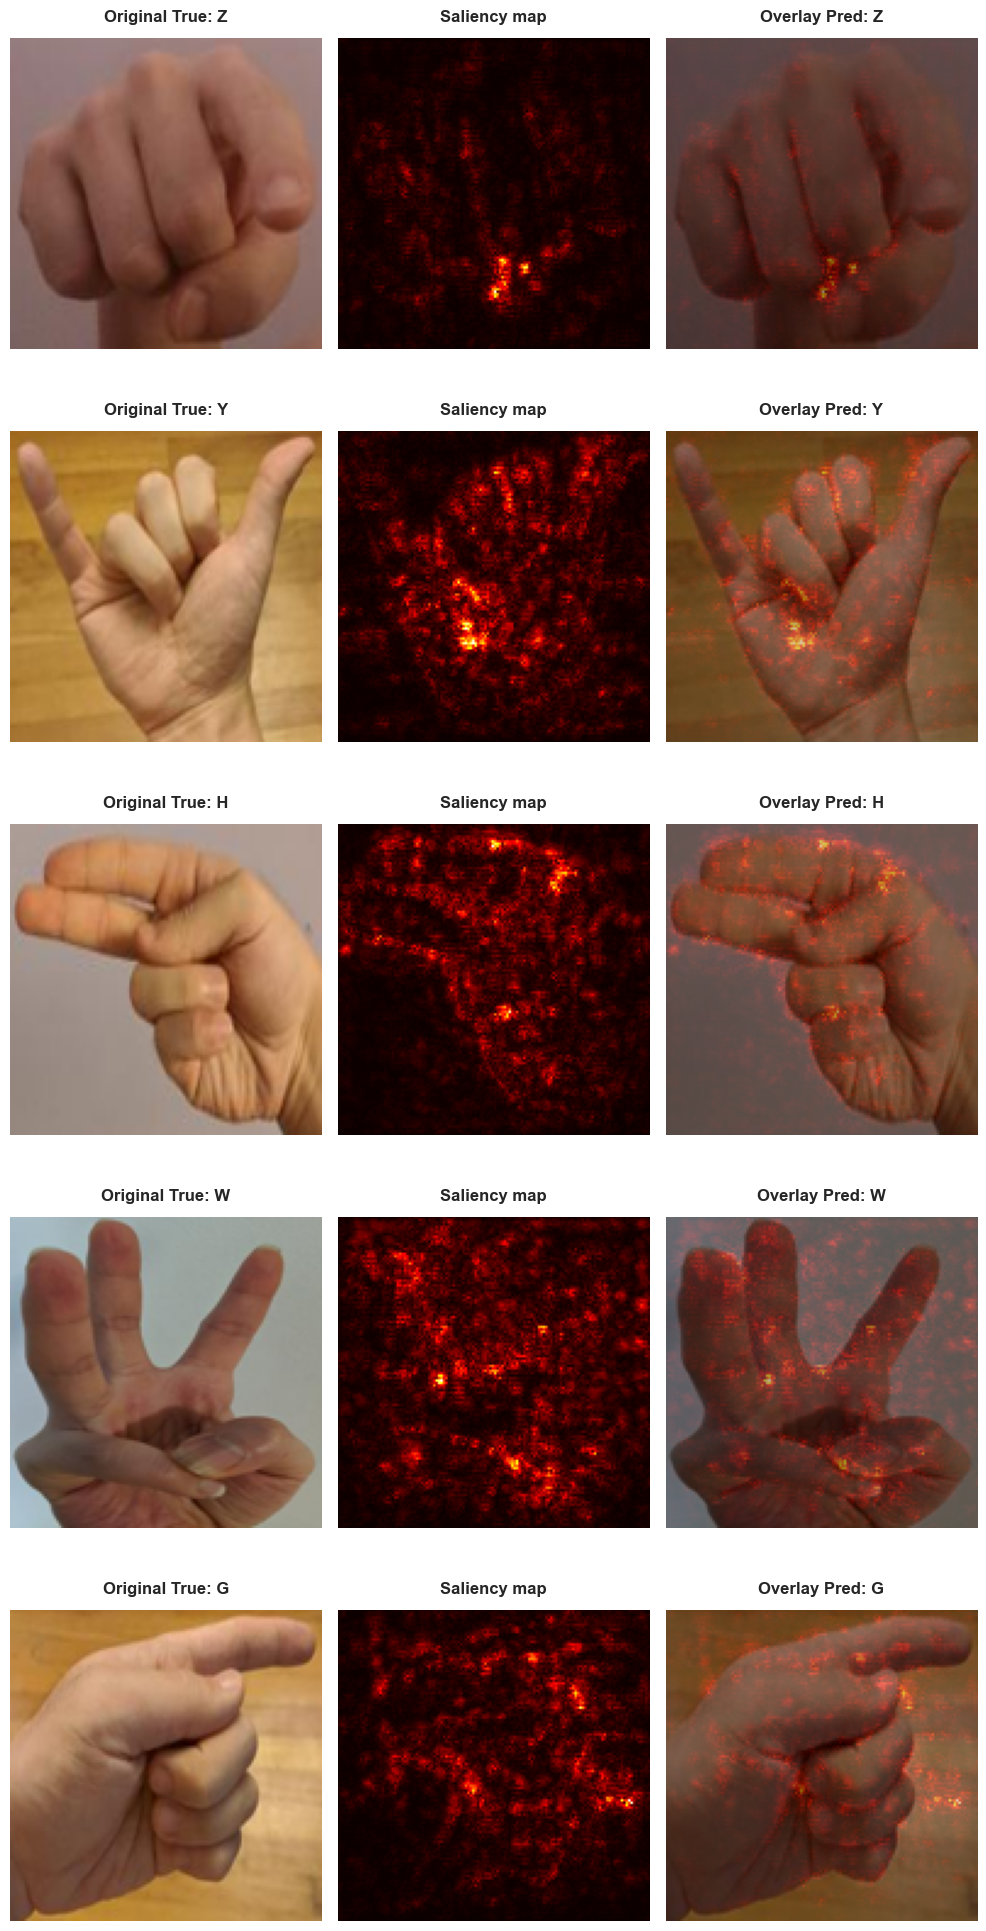
\includegraphics[width=0.82\textwidth]{report_figures/cell_80_0.png}
    \caption{Saliency map examples for test images.}
\end{figure}

\begin{figure}[H]
    \centering
    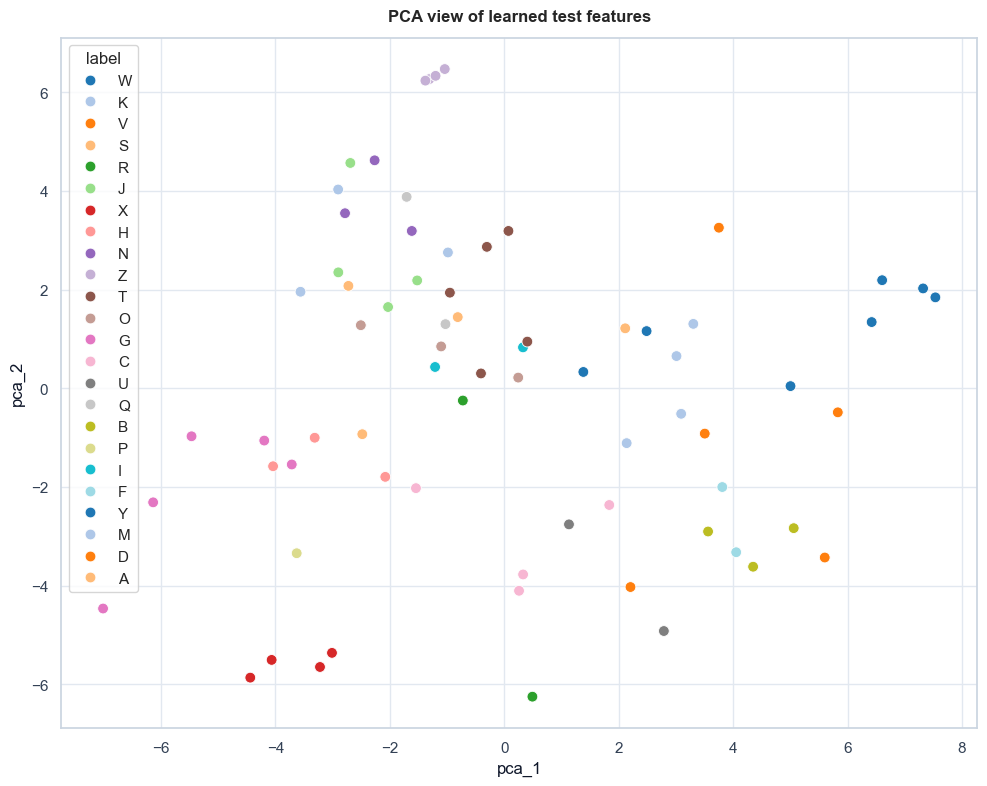
\includegraphics[width=0.78\textwidth]{report_figures/cell_83_0.png}
    \caption{PCA view of learned test features.}
\end{figure}

\begin{figure}[H]
    \centering
    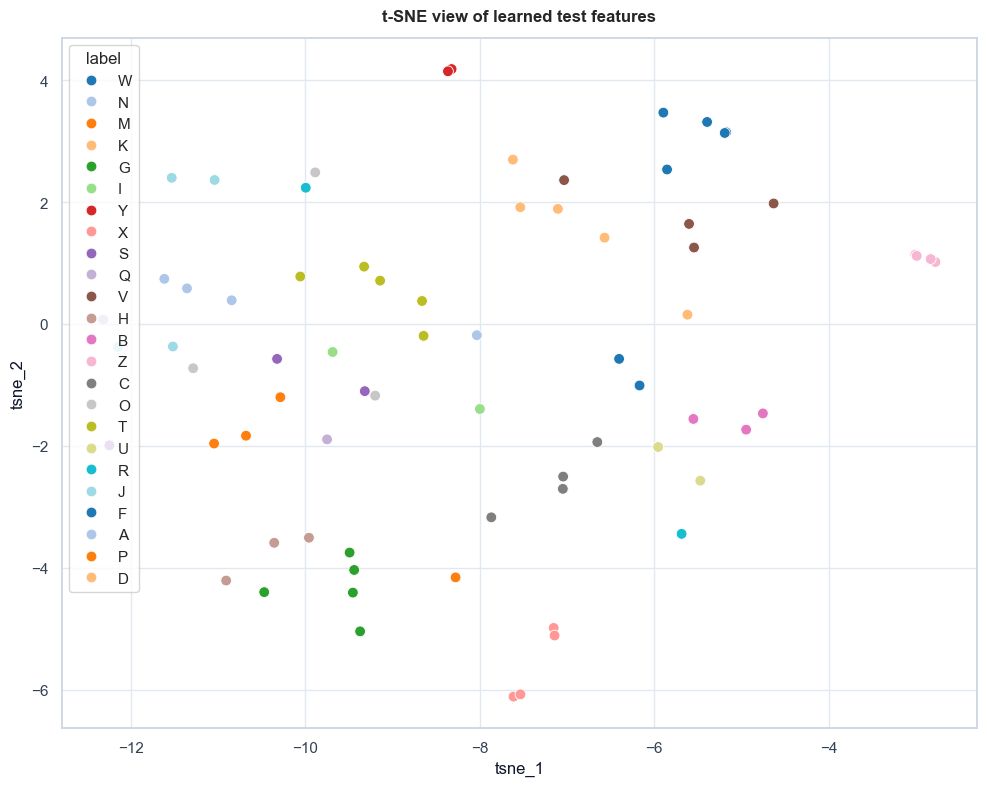
\includegraphics[width=0.78\textwidth]{report_figures/cell_84_0.png}
    \caption{t-SNE view of learned test features.}
\end{figure}

\begin{figure}[H]
    \centering
    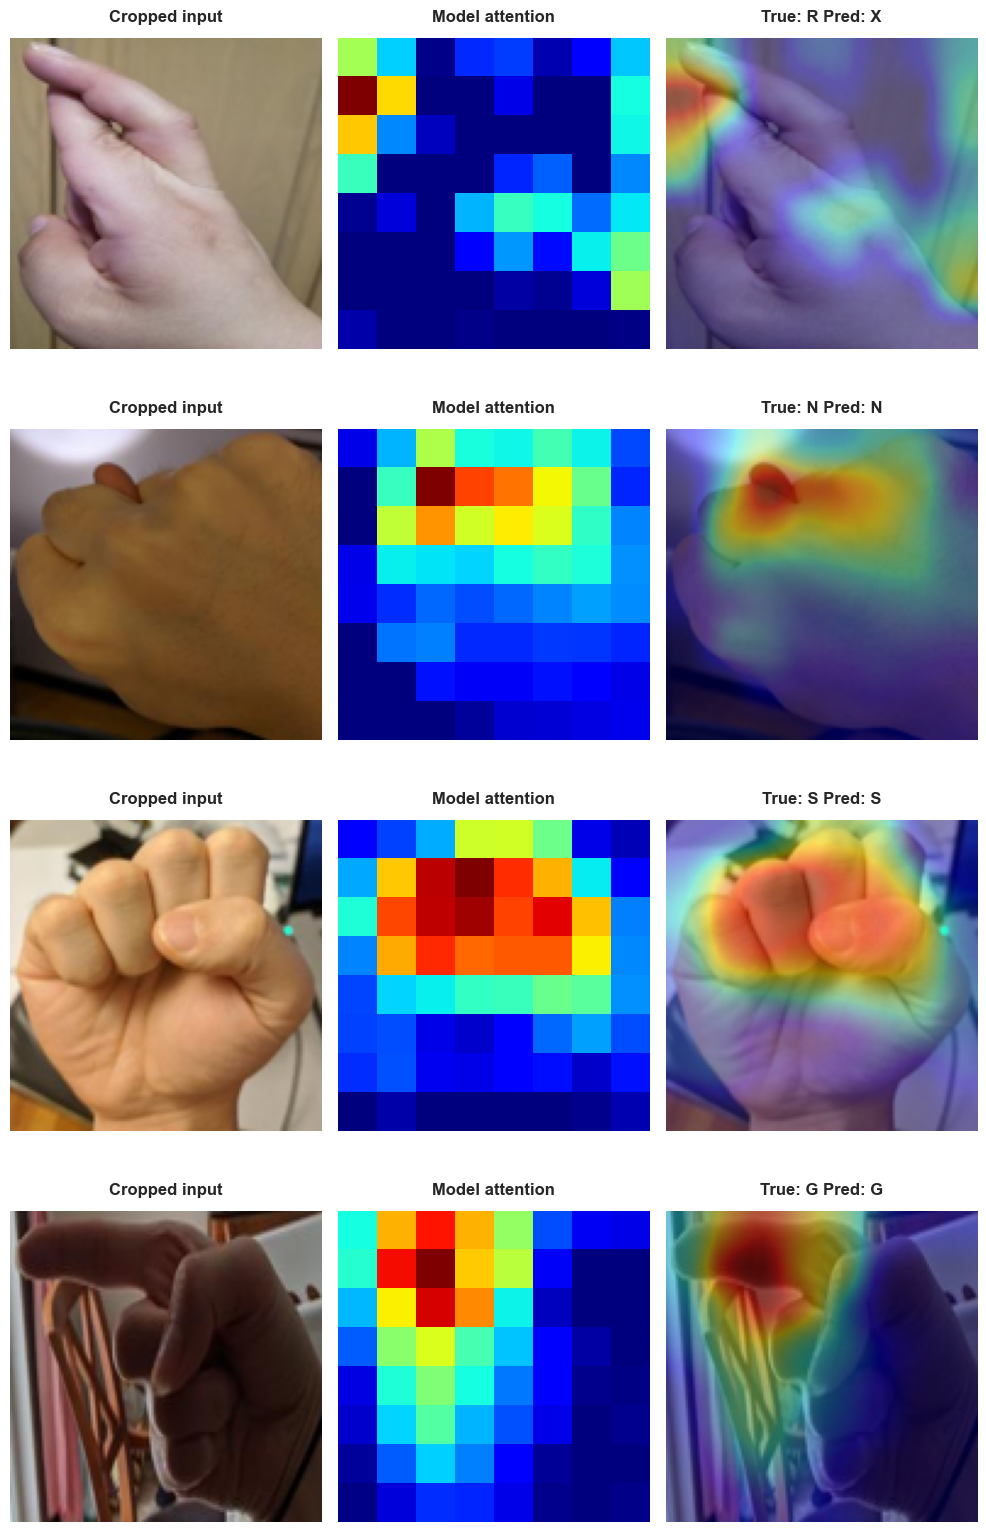
\includegraphics[width=0.8\textwidth]{report_figures/cell_86_0.png}
    \caption{Comparison between cropped inputs, heatmaps, and overlay results.}
\end{figure}

\qtext{What is the final comparison and conclusion?}

\ansstart
I tried more than one setup, but only one model reached the best test accuracy. So my final chosen model is the first main PyTorch CNN with test accuracy \textbf{86.11\%}. The later four-model search gave useful comparison results, but none of those models beat this test score.

The main trade-off I saw was simple. The more regularized model got the best validation accuracy, but it did not give the best test accuracy. So for this assignment, I cared more about test accuracy and kept the stronger test model as the final answer.

Overall, the preprocessing pipeline worked well. Cropping removed useless background, resizing to 128 \(\times\) 128 kept enough detail, normalization made the inputs stable, and training-only augmentation helped the model handle variation. The final CNN gave strong accuracy and the extra plots helped explain both the strengths and the mistakes.
\ansend

\section{Notebook Figures Used in the Report}

\qtext{Which notebook images were used?}

\ansstart
I used all of the plot images that were saved from the notebook outputs, plus the model graph and the runtime screenshots that were already in the project folder.
\ansend

\begin{figure}[H]
    \centering
    \includegraphics[width=0.58\textwidth]{images/x2.png}
    \caption{Runtime snapshot from training on my machine.}
\end{figure}

\begin{figure}[H]
    \centering
    \includegraphics[width=0.58\textwidth]{images/x3.png}
    \caption{Another runtime snapshot while running experiments.}
\end{figure}

\begin{figure}[H]
    \centering
    \includegraphics[width=0.58\textwidth]{images/x1.png}
    \caption{Hardware usage snapshot during CNN training.}
\end{figure}

\end{document}
